\documentclass{ltjsbook}
\usepackage{docmute} 
\usepackage{../../myStyle} 

\begin{document}
\chapter{帰無仮説検定の注意点}
\label{ch14_NHST2}
さて前回は帰無仮説検定について説明しましたが，いかがだったでしょうか。
まず「関係がない」「差がない」といった\keytermL{帰無仮説}{きむかせつ}をおき，本来主張したいことを\keytermL{対立仮説}{たいりつかせつ}とし，帰無仮説の否定をもって対立仮説の採択とする，という\textbf{背理法}のロジックで結論を導き出しますから，少しひねくれた考え方になっていることに注意が必要です。手元に得られたデータが，帰無仮説の下では滅多に生じ得ないことだということでもって，帰無仮説を棄却するということも理解していただいておりますでしょうか。

今回は，この帰無仮説検定を行った結果を，どのように報告し，どのように解釈するのかについての解説を行います。とくに解釈の仕方については注意が必要で，少し触れたように帰無仮説検定は\textbf{誤用・誤解が多い}ことも指摘されています。筆者の考えでは，背理法というひねくれた考え方と，基準となる確率の考え方が不自然であることに根本的な原因があり，初学者には帰無仮説検定は向いてないのではないかとさえ思います。それでもその手軽さから広く浸透した手法ですから，皆さんが先行研究などで触れる過去の論文の中にも間違った使い方，間違った解釈をしているものが含まれているかもしれません\footnote{プロの研究者(大学教員など)が書いて，プロの研究者が査読して刊行されている学会論文においてさえ，間違った手法や解釈が含まれている可能性があります。一つは時代的なもので，かつて計算機が十分に発達していなかった頃には正しい分析法が適用できず，やむなく代替案・次善の策として別の方法を使わざるを得なかった，という事情です。当時は正しいとされていた分析手法が，のちの研究で問題が指摘され，より改良された正しい方法ができることもあります。いずれにせよ研究をする上では，常により正しい手法を使うように心がけなければなりません。また，正しくない手法と知りながら実践するような態度は厳に慎まなければなりません。}。皆さんが同じ過ちを犯さないように，しっかりと基礎知識を身につけ，安易で誤った答えに飛びつかないようにしてください。

\section{有意水準と$p$値の解釈}

先の章では，相関係数と$\chi^2$値の検定，平均値がある値であるかどうかの検定(一標本検定)をみてきました。どちらも帰無仮説と対立仮説を立て，検定統計量を計算し，その値が有意水準を上回るかどうかで棄却・採択を判断するという流れでした。データの種類や統計量にかかわらず，帰無仮説検定の手順は同じ手順を踏みますので，このようにマニュアル化することができます。そのおかげもあって，心理学をはじめとして多くの領域で検定が行われるようになりました。実際，統計パッケージには検定をするための関数やメニューがあり，ジャンルが心理学であれ経済学であれマーケティングであれ生物学であれ，とにかく尺度水準や検定統計量の選定を間違えなければ検定はできるというわけです。また，検定の結果「有意である」となれば「差がある」「効果がある」といった結論にお墨付きがもらえるように思えるのも，検定が広く使われる理由の一つです。

しかし，検定の結果が有意であるということは，必ずしも意義のある結果であるというわけではありません。あくまでも「\underline{統計的に}有意である」ということであり，「実社会において\underline{意味(意義)}がある」ということではないのです。この辺りは誤解や誤用が多いところなので，しっかりと注意しておきます。

まず，検定は「誤った判断をしない」ことを目的にしています。確率的な判断なので確実に間違えないことは無理ですが，せめて「効果(差)がないのにあると判断する」ことを避けよう，というのが検定の目的です。
100\%の確率で間違えない，というのは無理ですが，5\%の確率で間違えることを許容する，というのが有意水準です。つまり，帰無仮説検定は「帰無仮説が正しいときに，それを棄却してしまう確率を5\%以下に抑える」ということを目的にしています。

また，帰無仮説検定は判断のためのツールであることを忘れてはいけません。データからはいろいろ考えられることがありますが、その中で仮に「帰無仮説が正しかったら」という`if'の世界を考えて，これに対抗する「帰無仮説が正しくなかったら」という`if not'の世界との\textbf{モデル比較}をしているのです。その時の勝負の判定基準が有意水準です。ですから$p$値が有意水準を下回った(=効果があった，差があった)というのも，あくまでも`if'世界の話であって，現実世界の話ではないのです。また，勝負がつくかどうかの判定であって，モデルの強さや正しさを表現する数字ではありません。

野球に例えていうならば，検定は遠くに飛んだ打球がフェンスを超えたかどうか，という判断をしているだけであり，ホームランの打球がどれぐらい速かったか，どれぐらい遠くに飛んだか，ということを表現しているわけではありません。ホームランの打球が速いかどうかは，別の指標である打球速度や飛距離で表現されるはずですし，打者が優れているかどうか，チームが強いかどうかという話ではないのです。

なぜこのように口やかましくいうかというと，上で挙げたような誤解が少なくないからです。\textcite{Wasserstein2016}では，$p$値について次の6つの原則をあげています。
\begin{enumerate}
	\item $p$値は、データが特定の統計モデルとどの程度両立しないかを示す
	\item $p$値は仮説が真である確率や、データが偶然によって生成された確率を測定しない
	\item 科学的結論は、$p$値が特定の閾値を超えるかどうかのみに基づくべきではない
	\item 適切な推論には完全な報告と透明性が必要
	\item $p$値や統計的有意性は、効果の大きさや結果の重要性を測定しない
	\item $p$値単独では、モデルや仮説に関する証拠の良い尺度を提供しない
\end{enumerate}
このような警句を発しなければならないほど，$p$値や有意水準の使い方が誤解されているということです。心理学では，このような誤解を避けるために，検定の結果を報告する際には有意水準を明示することが求められています。たとえば「$p<.05$」といった形で，どの有意水準で検定したかを明示するのです。

また，結果の報告だけでなくその解釈において，$p$値が小さければ小さいほど良いとか，$p$値が小さい方がより強い・正しい仮説であることを意味する，といった解釈は明らかに誤りです(でもときどきそのような表現を見かけます)。$p$値は帰無仮説が正しいという仮定の世界での値であり，現実の世界での正しさや正確さを表現しません。ある意味，帰無仮説は常に正しい(仮定しているのだから)わけであり，$p$値の大きさに一喜一憂する必要はないのです。

同様に，有意水準の設定にも注意が必要です。心理学では5\%水準がよく使われますが，これはあくまでも習慣的なものであり，1\%の方が厳しい検定をした(それを潜り抜けたから，より強い証拠が得られたと言える！)というわけではありません。基準は6\%でも4\%でも10\%でも構わないのです。たまに，5\%水準で検定をしたが有意にならず，$p$値を見ると0.06「おしい」ので，「有意傾向にあった」という表現を見かけることがあります。これは「もうちょっとでホームランだったのに」と言ってることと同じで，「もうちょっとでホームランだったから，点数が入ったものとして考察する」というのはおかしなことなのです。

\section{統計的に有意とは}
\label{sec:14_01}

あらためて考えると，「統計的に有意statistically significant」とはどういうものでしょうか。

相関係数の検定の時のことを思い出しましょう。帰無仮説は$\rho=0$というものでした。これが棄却されたので，「統計的に有意な相関係数だ」と結論づけたわけですが，より正しくは「母相関が0であるとはいえない」ということですよね。関係がないとは言えない$\to$関係がある，というこの$\to$の部分は，厳密に言えば少し飛躍があることになります\footnote{「あなたのことが嫌いではない」といわれても好きだとは言われてないわけで。}。

この帰無仮説検定を考えた人は，R.A.フィッシャーという人なのですが，この人は帰無仮説が棄却されたら「なにかおかしなことが現実に起こっているのだから，実験手続きを見直したほうがいい」というチェックのために使うことが想定していました。これをE.ピアソンとJ.ネイマンという人が「帰無仮説の棄却＝対立仮説の採択，とすれば良い」という判断基準と合わせて使う方法へ応用したのです。心理学ではその流れを受けて帰無仮説検定を利用してきました。そういう意味で，本来の創始者の意図とは違った，より実践的な意味のある(言い換えれば実用上の責任を負わなければならない)使い方をしているのです。

また既に述べたように，実際の相関係数の大きさや，平均値の差についての情報がかき消された表現になっていることにも注意が必要です。最終的な判断は$p$値だけを見るのですが，この数字だけみても相関係数の大きさや，平均値の差がどれぐらいあったのかはわかりません。有意になったという結果だけをみて，関係があったのか，そうかー，と考察を巡らせても，実は標本相関係数が$r=0.1$だったということもありえるのです\footnote{実際に，サンプルサイズが271人を超えると，標本相関係数が$0.1$でも5\%水準で有意になります。}。これで「統計的に有意だ！無相関とは言えない！」と言っても，標本相関係数が0.1なのですから，「(相関)関係がある」という結果をもとに議論するとおかしなことになってしまいます。

ところが実際，このような表面上の使われ方に引っ張られてしまうことはよくあります。とくに研究をしていると，努力したのに関係がなかったとは\underline{言いたくない}という気持ちが働いてしまいます。そこで，有意になったんだから意味はあるよね，と考えて無理やり二変数間の関係を考察してしまう，ということになってしまいます。これではせっかくデータを取ったのに，正しく考えられたことになりません。

一般にサンプルサイズが大きいと，$p$値は小さくできますから，帰無仮説は棄却しやすくなります。図\ref{fig:14_01}には，横軸にサンプルサイズ，縦軸に$p$値をとり，標本相関係数が$r=0.5,0.3,0.1$のときにどうなるかをプロットしました。5\%を有意水準(点線)としていますが，サンプルサイズが大きくなるにつれて$p$値は小さくなって行きます。

\begin{figure}[ht]
	\centering
	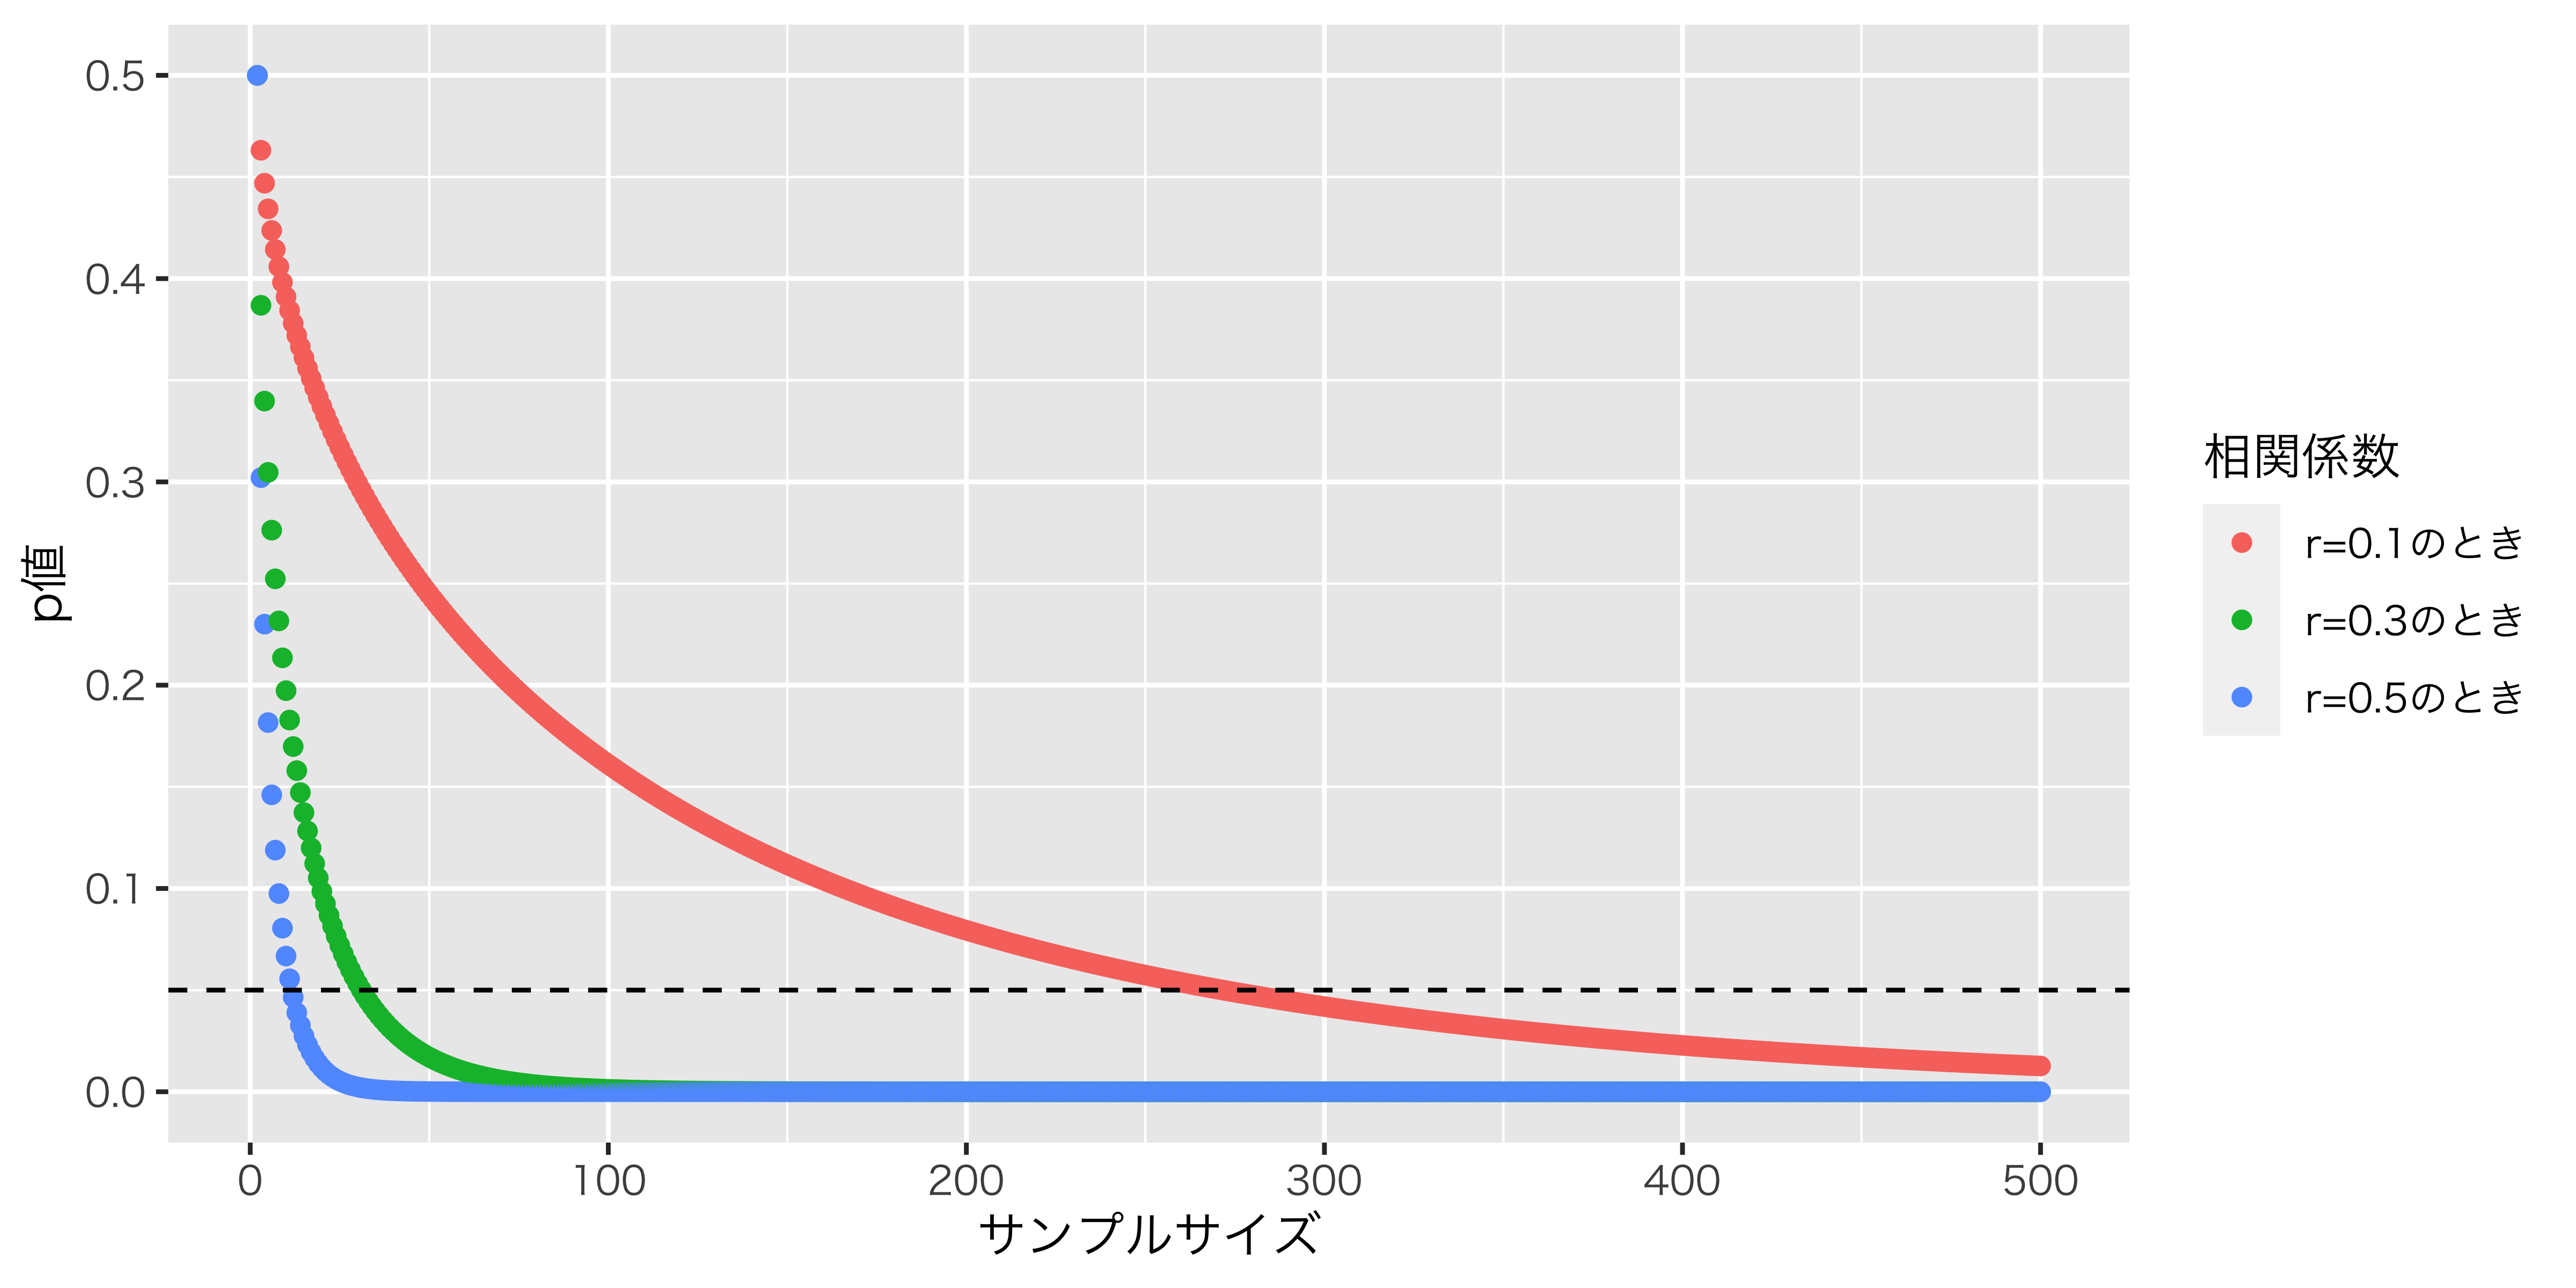
\includegraphics[keepaspectratio,width=0.8\linewidth]{figures/14_NHST2/p_value_curve.png}
	\caption{サンプルサイズと$p$値の関係}
	\label{fig:14_01}
\end{figure}

この下がり方はどこからスタートするかにかかわらず同じ形ですから，判定はサンプルサイズが増えさえすればいずれ有意になるのです。これがまた，研究の実践ではおかしな風潮を呼んでしまいます。つまり，\underline{有意にしたければ}サンプルサイズをたくさん取る＝頑張れば良いのです。

しかしながら，科学的に正しいかどうかを考えるべきシーンで，「頑張れば有意になる」といった``努力''に依存するのはおかしいことだと思いませんか。頑張った$\to$有意になった$\to$著者の主張が正しい，というのは，論理的ではありません。結果を自分の都合の良いように変えることは，正しい努力ではないはずです。

帰無仮説検定は，標本から母集団のことを「判定」できる優れた技術ですが，表現とその解釈に気をつけないと，科学を間違った方向に導きかねないことに注意が必要です。残念ながら，これまでの心理学の歴史の中でもこのような間違った努力がなされてきた事実があります。これらは\keyterm{問題のある研究実践}{もんだいのあるけんきゅうじっせん}{Questionable Research Practices}，すなわち\keytermL{QRPs}{QRPs}と言われています。たとえば「有意な結果にするために」サンプルサイズを増やすとか，「有意な結果になるまで」検定を繰り返す，といったことがQRPsに当たります。そうした研究実践が実際に行われている現場も少なくないようです。しかしそんなことをしていると，必然的に科学の議論が「正しくない結果(の解釈)」に基づきますから，後続の研究が土台から崩れ，長年の努力が無駄になってしまいます。データの捏造や，他人の書いた論文を盗む剽窃は明らかに悪意のある行為ですが，「頑張ってデータを増やす」というのは一見真面目で誠実な研究態度に思えてしまうので，ちょっとタチが悪い問題です。努力が人を誤らせるのですから。皆さんも騙されたり間違った道に進んでしまわないよう，十分に注意して研究を進めてください。

\section{検定における2種類の間違い}
\subsection{$p$値とは何か}
\label{sec:14_02}
ところで，帰無仮説検定は「推定」の応用である「判断」だということでした。判断が確率的に行われるのですが，人間は確率的な考え方が得意ではありませんから，うっかり間違って理解してしまうことも少なくありません。正しい判断，間違った判断というのはどういうときに起こるのかを考えてみましょう。実はこれも，確率的表現の難しさがあるのです。


% まず先ほどから$p$値と呼ばれる数字を使って説明してきましたが，改めてこの$p$値は何を表している数字でしょうか？ 次の選択肢の中から考えてみてください。

% \begin{itemize}
% 	\item 帰無仮説の成立する確率
% 	\item 帰無仮説の正しさを表している数字
% 	\item 有意の程度の強さを表している数字($p$値が小さければ小さいほど効果が大きい)
% 	\item 検定の強さを表している数字
% \end{itemize}

% 実は正解は，上のどれでもない，です。意地の悪い選択肢でごめん。

% 上の2つの選択肢，「帰無仮説の生じる確率」「帰無仮説の正しさを表している数字」はよくある勘違いです。
% 仮説検定は「帰無仮説の下で・・・」という前提から始まります。無相関検定のときに，母相関が0の世界から標本をピックアップする例をお話ししましたね。母相関の世界を前提として・・・という話なので，帰無仮説の生じる確率は100\%，帰無仮説の正しさも100\%です(だって仮定したんだから！)。

% 有意の程度の大きさを表す数字でもありません。確かに差が大きいとか，帰無仮説の世界から大きく離れているというようなことがあれば，検定統計量の実現値は大きくなり，$p$値は小さくなります。が，$p$値が示しているのは\underline{(帰無仮説の下での)検定統計量の出現確率}に過ぎません。いわば帰無仮説という仮想空間の中での数字であって，現実の統計量について何か示す数字ではないのです。

% 検定の強さを表す数字，でもありません。$p$値が小さくなればなるほど，確かにレア度は増しているのですが，それは帰無仮説という仮想空間の中でのレア度であって，帰無仮説が対立仮説をどれほど打ち負かしたか，という情報を持っているわけではありません。ですから，$p$値が小さければ小さいほどすごい，などと思ってしまうと本質を見誤ります。

帰無仮説検定最後のステップでは「最初に定めた仮説を支持するかどうか判断する」というのがありました。この判断の間違い方にも，2種類あることになります。つまり，「帰無仮説が正しいのに棄却してしまう」という間違い方と，「帰無仮説が正しくないのに採択してしまう」という間違い方です。

\begin{figure}[ht]
	\centering
	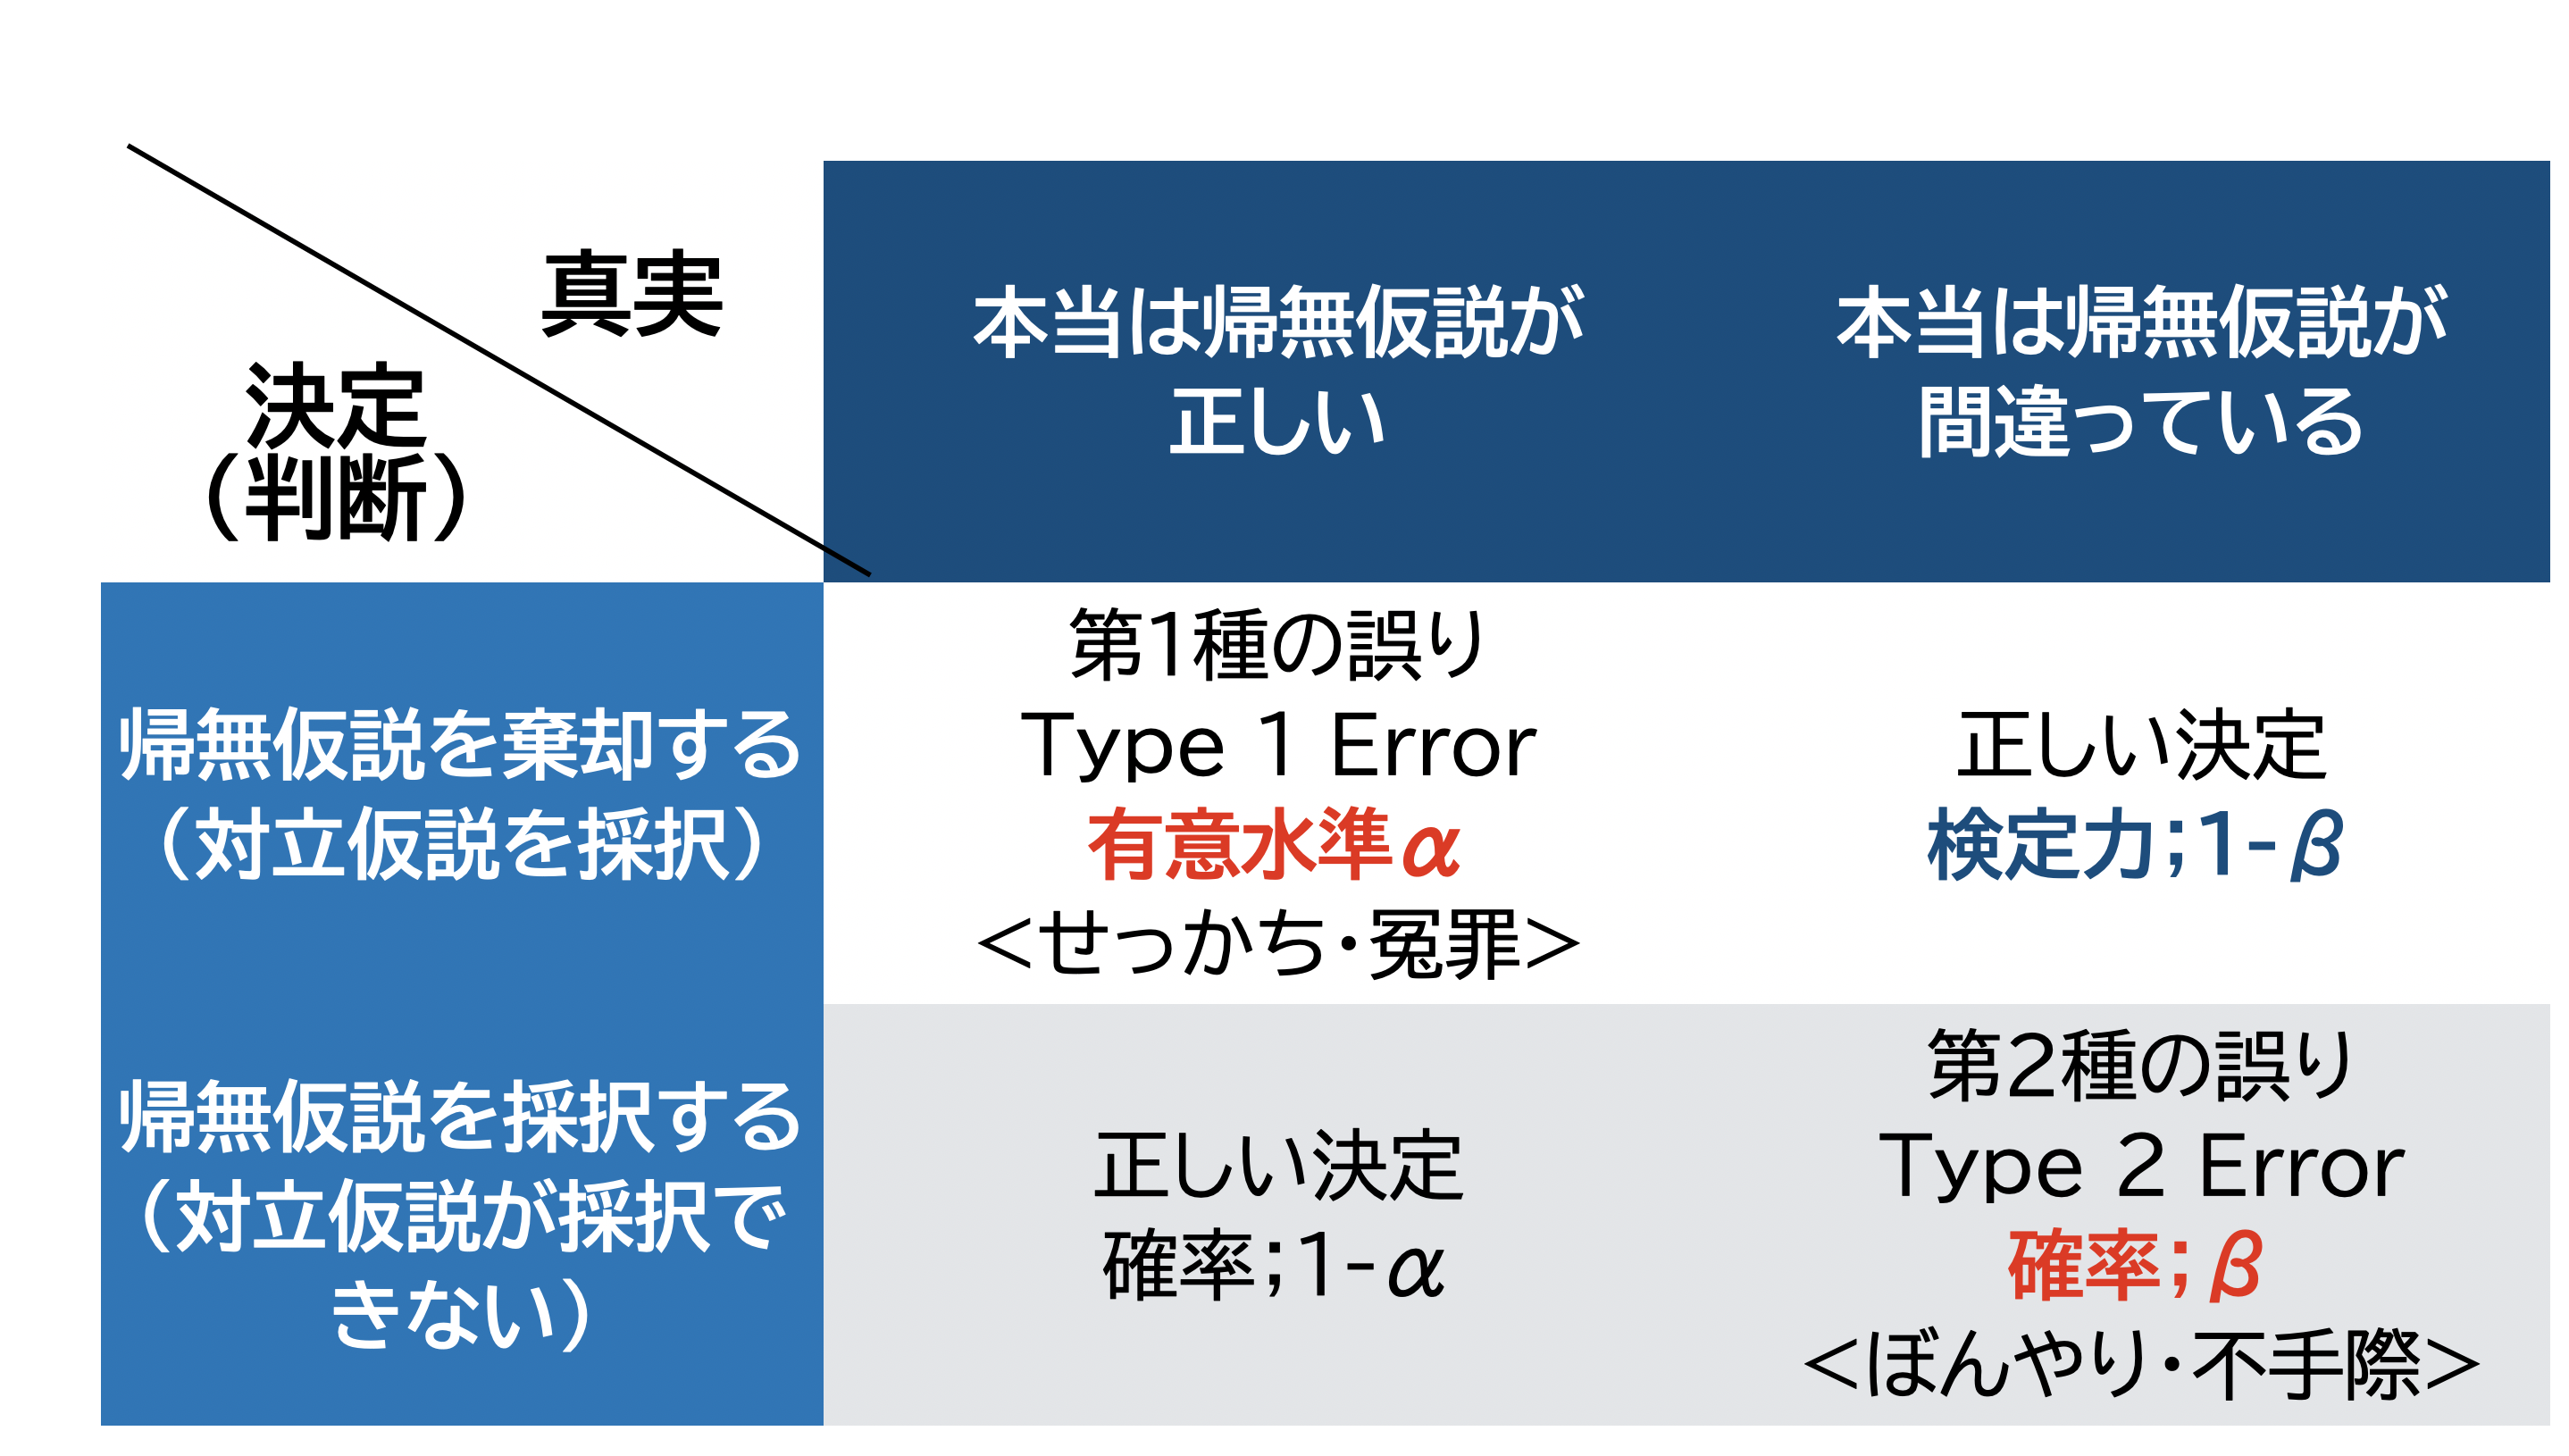
\includegraphics[keepaspectratio,width=0.8\linewidth]{figures/14_NHST2/type12.png}
	\caption{二種類の間違い方}
	\label{fig:14_02}
\end{figure}
図\ref{fig:14_02}に，間違い方の組み合わせを書いてみました。帰無仮説が正しいときに帰無仮説を採択する，帰無仮説が正しくないので帰無仮説を棄却する。これができれば正しい決定ですが，「帰無仮説が正しいのに帰無仮説を棄却する」のも「帰無仮説が正しくないのに帰無仮説を採択する」のも間違いです。

帰無仮説は差がないとか効果がないといったからっぽ(Null)な結論です。ここでは仮に，開発された新薬に治療効果があるかどうかを考えている，というシーンを想像してみてください。帰無仮説はこの新薬に効果がないときです。ロクな効果がないときに，帰無仮説を棄却する＝対立仮説を採択する＝効果があると言ってしまうのは，怖いことですね(患者さんに副作用など悪影響があるかも！)。このような功を焦って誤った判断をしてしまう危険な間違いを，\keyterm{タイプ1エラー}{たいぷ1えらー}{Type I Error}とよび，その確率を$\alpha$で表します。実は，5\%水準で判断するというのは，この$\alpha$の確率を0.05にしたことになります。慣例では$\alpha=0.05$となっていますが，別に1\%でも10\%でも，自由に決定して構いません。どの程度の水準にするかは，この間違いを犯した時の重要さを参照しながら決めるべきことです。

一方，効果があるのに(帰無仮説が間違ってるのに)，帰無仮説を採択するのは，せっかくの効果を見抜けなかった残念なケースです。これも困った結果ではありますが，少なくとも患者に迷惑がかかるようなことはありませんよね。なので，こちらについてはひとまず間違っても実際的な問題は生じないでしょう。こちらのケースは\keyterm{タイプ2エラー}{たいぷ2えらー}{Type II Error}と呼び，確率は$\beta$で表すのが一般的です。ただ，この$\beta$は帰無仮説が間違っている，つまりNull「でない」状態が，どう「である」のかわからないので，大きさを見積もることはできません。せめて，効果があるときはちゃんとあるって知りたいよね，と思いを馳せるだけです。この図\ref{fig:14_02}にある表は，列ごとに世界線が分かれていますから，右列の「帰無仮説が間違っている世界」で「帰無仮説を棄却してしまう確率」が$\beta$であれば，ちゃんと効果を見つけ出せる確率は$1-\beta$です。この$1-\beta$を\keyterm{検定力}{けんていりょく}{power}といい，検定力のある分析ができているかどうかをちゃんとチェックしておくのは，研究の手続き上重要なことです。

すでに述べたことですが、帰無仮説検定は$\alpha$水準を一定に保つことを目標にしています。$\beta$の方は「本当はどれぐらい差があるのか」がわからないので，コントロールのしようがないのです。事後的に，今回の$\beta$はどれぐらいだったのかな，と考えることはできませんが，事前に調整することはできません。ですからせめて，$\alpha$の方はコントロールしておきましょう，というのが帰無仮説検定の基本的な考え方なのですが，実はここにも注意が必要なのです。

\subsection{$\alpha$のインフレ}
\label{sec:14_03}
先ほど，5\%水準という\keytermL{有意水準}{ゆういすいじゅん}は$\alpha$を設定したことと同義だという話をしました。つまり効果がないのに効果があると言ってしまう，うっかりミスを防いでおこうという方針で判断基準を設計しておきましょうということです。
それを踏まえた上で，次のような話を考えてみてください\footnote{この例え話は\textcite{BA33892274}からの引用です。}。
\begin{quote}
	あるレストランの地下にはたくさんのワインが貯蔵されているが，20本に1本は酸っぱくなった不良品が混じっている。客がやってきて1本のワインを注文する時，ソムリエは長い目で見て20回に1回冷や汗をかくことになる。
	このレストランで開かれるパーティには10本単位でワインを出すことになっているが，1本でも酸っぱいワインが入っていたらパーティはダメになってしまう。パーティーのときは，ソムリエはどれほど謝らなければならないか？
\end{quote}

何だか怪しいレストラン，いかがわしいソムリエですね。こんな店が実在していたら行きたくないですが，もちろんこれは架空の話で，20本に1本のダメなワインがあるというのは，帰無仮説検定における5\%の有意水準のメタファーになっています。
つまり，5\%の判断ミスが生じる危険性がある，ということですね。
うっかりミスの水準を5\%にしているのは，言い換えると95\%の高確率で判断があっているのですから，ほとんどの場合は問題ないとも言えます。このレストランでは20回に1回しかミスはない，というわけです。

ところがパーティーが開かれると，ワインがまとめてどっさり提供されるのでした。1回のパーティで10本のワインが出るんでしたね。
ひとまず2本のワインを持ってきたとします。危険率は5\%，安全率は95\%ですが，これは一本あたりの話です。2本連続で安全である確率は，$0.95\times 0.95=0.9025$になります。言い換えると，どちらか一本がアウトである確率は$1-0.9025=0.0975$で，なんとほとんど10\%ではありませんか。

同じように考えて，10本まとめて持ってくると，その中のどれか一本でも間違っている確率は，$1-(0.95)^{10}=0.4013$ということになります。40\%ですね。
つまり10本まとめて持ってくると，一本ずつだと5\%だった危険率が40\%に跳ね上がっていることがわかります。

話を心理学の世界に戻しましょう。心理学では実験の結果を検証するときに，5\%の危険率で判断するのでした。
さて，とある熱心な研究者がある現象についてさまざまな角度から研究し，何度も統計的な検定を重ねて結論を導き出そうとしているとします。その研究者はとても熱心で慎重なので，1つの研究のなかに10種類の実験を考え，10回それぞれ5\%水準で帰無仮説検定を行い，丁寧に判断を繰り返してすべて有意な効果が得られたとします。これは頑健な結果だ，一連の研究はうまくいったぞ・・・といえるでしょうか。

実はそうならないのです。さきほどのワインの話のように。つまり1つの研究で10回検定を行うと，たまたまどこかで有意になる(差がないのに差があるように判断してしまう)可能性が40\%に膨れ上がっています。
つまり，一連の研究で5\%の危険率を維持しようとするなら，たとえば10回の検定が含まれるのであれば，それぞれの有意水準はせめて0.5\%にしておかなければなりません。さもないと，うっかりミスの確率がインフレしてしまうのです。

これも悲しいかな，努力が裏目に出てしまう可能性ですね。一見，1つの論文で複数回の実験や検定を行なっているのは，慎重で真面目であり，有意な結果が出ればそれは十分強い証拠だ，と考えてしまいます。しかしこれはあくまでも0/1の判断であり，しかも確率的な判断ですから，間違いの評価の仕方も確率の理論に沿って丁寧に考えねばなりません！

実際ひとつの論文の中に複数回の検定が行われていることは，少なくありません。しかしその中で，$\alpha$水準の全体的な調整がなされていることはあまり見かけません。そう，多くの研究者は気づいていながら間違った研究実践をしているのです。「みんな間違っていてみんないい」とはならないのでして，こうした状況は一刻も早く修正する必要がありますが，なぜかなかなか浸透しないところでもあります。本来は，1つの論文全体で調整をかけるべきなのですが・・・。
こうした誤りに振り回されないようにするには，「差がある/ない」といった1 bit判断にするのではなく，「どの程度の」差が見られたのか，その効果の大きさをしっかり見極める目が必要になってきます。


\section{効果量と例数設計}
\label{sec:14_04}
検定力のチェックは，分析が終わった後に事後的にすることもできますし，事前にすることもできます。事前に，というのは，みたい効果がどの程度あるのかを考え，その効果をきちんと検出するにはサンプルサイズをどれぐらいにすれば良いのかを考えること，でもあります。このサンプルサイズを考えることを，\keyterm{例数設計}{れいすうせっけい}{sample size design}といいます。

帰無仮説検定において，例数設計はとても大事なことです。既に述べたように，サンプルサイズが大きくなると有意だという判断はしやすくなります。これは$p$値で判断する以上仕方のないことですが，だからと言ってそれを逆手にとって，事実よりも主張をするためにサンプルをたくさんとるのは，帰無仮説検定のハッキングのようなものです\footnote{実際これを\keytermL{p-hacking}{p-hacking}と呼ばれるよくない研究実践の典型例です。}。ですので，検定をするときはまず「どの程度の効果が見込まれ，これを検証するためには何人ぐらいのサンプルをとらなければならない」と宣言してから，検定して判断するという手続きが必要です。この宣言をせずに検定をすると，「有意にするためにサンプルサイズを変えたのではないか」と批判されてしまうかもしれません。学部の授業や卒論で行う実験で，例数設計をしたりサンプルサイズの宣言をするようなことはないかもしれませんが，学術業界では事前に学会にこの宣言を伝えてから研究に取り掛かる，事前登録制pre-registrationが導入されはじめています。

ここで，検定の判定結果に関係してくる要素を改めてみて思い出してみましょう。1つはもちろん\keytermL{有意水準}{ゆういすいじゅん}ですね。これは判定を決める基準ですから，これが緩いと対立仮説の勝ち！という結果が出やすいことになります。
2つ目は\keytermL{サンプルサイズ}{さんぷるさいず}ですね。サイズが大きければ区間推定の幅は狭くなりますから，たくさんデータをとれば取るほど対立仮説の勝ち！という結果が出やすいことになります。ここまではお分かりいただけていると思います。
続いて3つ目は，\keyterm{効果量}{こうかりょう}{Effect Size}です。平均値差の検定の場合を例に簡単に言えば，群間の差の大きさのことです。母集団において本当に平均値の差が大きければ大きいほど，対立仮説の勝ち！という結果が出やすいことになります。これは当然ですよね。ただ，効果量を一般的にいうと\textbf{標準化された差}という言い方をします。100点満点のテストで1点の差がある場合と，1000点満点のテストで1点の差がある場合は同列に考えることができないですから，標準偏差で割ることで「標準偏差何個分離れているか」という表現にするのです。標本から推定する効果量としては，\keyterm{Cohenのd}{Cohenのd}{Cohen's d}と\keyterm{Hedgesのg}{Hedgesのg}{Hedges's g}が有名です。Cohenのdは次のようにして計算します。

$$d = \frac{\bar{X}_1-\bar{X}_2}{\hat{\sigma}}$$

ここで分母の標準偏差は，2群で同じであれば問題ないですが，異なる場合は$\hat{\sigma} = \sqrt{\frac{\sigma_1^2+\sigma_2^2}{2}}$として合わせて計算します。
いずれにせよ，「本当に差が大きければ対立仮説が採択される」というのは当然そうあって欲しい性質ですから，これもお認めいただきやすいと思います。

そして最後にもう1つ。先ほどの二種類の間違いのうち，本当に差がある場合に正しく検出できる程度，つまり\keyterm{検定力}{けんていりょく}{power}というのがありました。うっかりミスである\keytermL{タイプ2エラー}{たいぷ2えらー}を犯す確率が$\beta$ですから，検定力は$1-\beta$です。これも大きければ大きいほど，正しく対立仮説を採択できます。
\begin{figure}[ht]
	\centering
	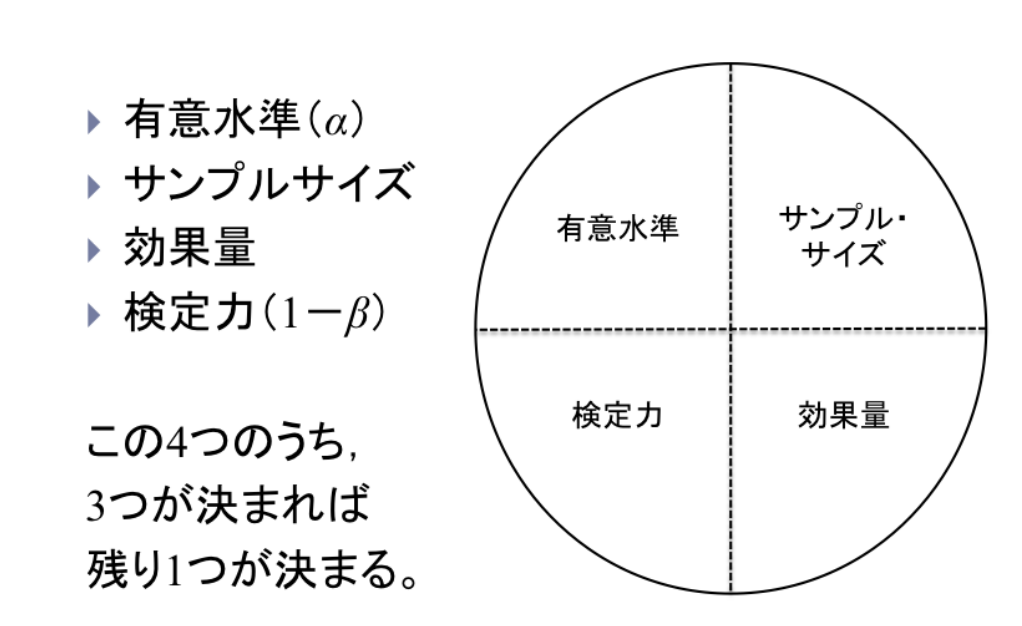
\includegraphics[keepaspectratio,width=0.8\linewidth]{figures/14_NHST2/conditions4.png}
	\caption{統計的検定における四つの要素の関係}
	\label{fig:14_03}
\end{figure}
このように，帰無仮説検定において判定に関係してくるのは有意水準，サンプルサイズ，効果量，検定力の4つであり，これらのうち3つが決まると残りの1つの要素は計算で決まります\parencite{Mizumoto2010}。また有意水準$\alpha$は一般に5\%を使いますし，検定力$1-\beta$も0.8ぐらいにするのがよい，というのが通例になっています。であれば，効果量に応じてサンプルサイズを決めることができるわけです。小さな効果しかなさそうなものであればサンプルサイズはたくさん必要ですし，逆もまた真です。ただ，「サンプルサイズは大いに越したことないだろう」というのは間違いで，そうすると実質的にはごくわずかな違いであっても，検定で検出してしまうことになるからです。
もっとも，研究を始める前に効果量がどれぐらいなのかを事前に知るのは難しいところです。効果がどの程度あるかがわからないので，研究しようというシーンが多いでしょう。それでも先行研究があれば，そこにはすでにサンプルサイズも，実際のデータによる効果量も計算できるわけですから，効果量がどれくらいある研究なのかを計算することは可能です。

研究を行う前に，事前にこれらの計算をすることを\keyterm{検定力分析}{けんていりょくぶんせき}{power analysis}と言います。検定力分析は，\keytermL{例数設計}{れいすうせっけい}をするためにも行われる場合と，研究後にどれぐらい効果量があったのかを調べる場合の二種類があります。またこうした計算をするための統計パッケージやRの関数などがありますので，実際はこれらを使って計算することになります。


\end{document}
